
\documentclass[12pt,a4paper]{article}
\usepackage[utf8]{inputenc}
\usepackage[T1]{fontenc}
\usepackage[brazil]{babel}
\usepackage{amsmath,amssymb,amsfonts}
\usepackage{graphicx}
\usepackage{booktabs}
\usepackage{hyperref}
\usepackage{minted}
\usepackage{tocloft}
\usepackage{geometry}
\usepackage{csvsimple}
\geometry{margin=2.5cm}

\title{PCS5029/PTC5725 -- Aula 05\\\large Introdução aos Métodos Espectrais (refações + tarefa)}
\author{Renan de Luca Avila}
\date{\today}

\begin{document}
\begin{titlepage}
\centering

\includegraphics[width=0.35\textwidth]{EP.jpg}\par\vspace{1cm}
{\scshape\LARGE Escola Politécnica da Universidade de São Paulo\par}
\vspace{1.5cm}
{\huge\bfseries Aula 05 -- Métodos Espectrais\par}
\vspace{0.5cm}
{\Large Refazendo exemplos de aula e Tarefa\par}
\vfill
{\large Renan de Luca Avila\par}
{\large \today\par}
\end{titlepage}

\tableofcontents
\newpage

\section*{Resumo}
Este relatório reimplementa, em Python, os exercícios apresentados nos slides da Aula 05 (Prof.\ Osvaldo Guimarães), e resolve o exercício da tarefa. O documento contém códigos completos, figuras e tabelas, além de apêndices com setup e fontes.

\section{Enunciados}
\subsection{Exercício 1 (refeito dos slides 2--3)}
Resolver a EDO não linear $u_{xx} - u^2 - 2 + (x^2-5x+6)^2 = 0$ com $u(-1)=12$ e $u(1)=2$ via Newton em grade de Chebyshev. Solução analítica $u(x)=x^2-5x+6$.
\subsection{Exercício 2 (refeito dos slides 4--5)}
Resolver $y''\,y + (y')^2 - 2e^{-2x}=0$ com $y(-1)=e$, $y(1)=e^{-1}$ via Newton-Chebyshev, utilizando 25 coeficientes e chute $y^{(0)}=\mathbf{1}$.
\subsection{Exercício 4 (tarefa da aula)}
Equação da difusão $u_t=C_d\,u_{xx}$ em $x\in[0,1]$, $t\in[0,T]$, com $u(0,x)=\sin(\pi x/2)$, $u(t,0)=0$ e $u_x(t,1)=0$. Método das Linhas (Chebyshev) + RK4. Comparar com a forma analítica do primeiro modo.

\newpage

\section{Resoluções}
Cada resolução é apresentada com planejamento, resultados, conclusão e implementação. Os códigos completos estão no Apêndice~\ref{ap:codigos}.

\subsection{Exercício 1 — EDO não linear (Colocação de Chebyshev + Newton)}

\subsubsection*{Enunciado}
Resolver a EDO não linear
\[
u''(x)\;-\;u(x)^2\;-\;2\;+\;(x^2-5x+6)^2 \;=\;0,\qquad
u(-1)=12,\; u(1)=2,
\]
cuja solução analítica é \(u(x)=x^2-5x+6\).
O objetivo é validar o método espectral de colocalização com polinômios de Chebyshev combinado ao método de Newton–Raphson.

\subsubsection*{Planejamento e fundamentos teóricos}
Representamos a solução por seus valores nos nós de Chebyshev–Lobatto \(x_j=\cos(\pi j/N)\), \(j=0,\ldots,N\).  
As derivadas são obtidas com a matriz diferencial \(D\) e seu quadrado \(D^2\).  
A formulação discreta da EDO é:
\[
F(u)=D^2u - u^2 - 2 + (x^2-5x+6)^2 = 0,
\]
e o Jacobiano associado é
\[
J(u)=D^2 - 2\,\mathrm{diag}(u).
\]
As condições de contorno são impostas fortemente nas linhas correspondentes a \(x=-1\) e \(x=1\), substituindo as equações por \(u(-1)=12\) e \(u(1)=2\).  
O método de Newton é então aplicado iterativamente:
\[
J(u_k)\,\Delta u_k=-F(u_k),\qquad u_{k+1}=u_k+\Delta u_k,
\]
até convergência (\(\|\Delta u\|_\infty<10^{-12}\)).

\subsubsection*{Etapas de implementação e funções principais}
O código em Python utiliza apenas \texttt{numpy} e \texttt{matplotlib}.  
A seguir são mostrados os blocos principais, comentados em linguagem natural.

\paragraph{1) Construção da matriz de Chebyshev (\texttt{cheb})}
\begin{minted}[fontsize=\small,breaklines,linenos]{python}
def cheb(N: int):
    """Matriz de diferenciação de Chebyshev-Lobatto e nós x."""
    if N == 0:
        return np.array([[0.0]]), np.array([1.0])
    x = np.cos(np.pi * np.arange(N+1) / N)
    c = np.ones(N+1); c[0] = 2.0; c[-1] = 2.0
    c = c * ((-1.0) ** np.arange(N+1))
    X = np.tile(x, (N+1, 1))
    dX = X - X.T
    D = (np.outer(c, 1.0/c)) / (dX + np.eye(N+1))
    D = D - np.diag(np.sum(D, axis=1))
    return D, x
\end{minted}

\noindent
\textit{Explicação:}  
A função gera os nós \(x_j=\cos(\pi j/N)\) e a matriz diferencial \(D\), que calcula derivadas espectrais por multiplicação.  
O quadrado \(D^2\) fornece a segunda derivada.  
Essa rotina segue a formulação clássica de Trefethen (1996).

\paragraph{2) Montagem do sistema não linear (\texttt{build\_system})}
\begin{minted}[fontsize=\small,breaklines,linenos]{python}
def build_system(u, D2, x):
    """Resíduo e Jacobiano do problema."""
    F = D2 @ u - (u**2) - 2.0 + (x**2 - 5.0*x + 6.0)**2
    J = D2 - np.diag(2.0*u)
    return F, J
\end{minted}

\noindent
\textit{Explicação:}  
Calcula o resíduo \(F(u)\) segundo a EDO e o Jacobiano \(J(u)\) usado no método de Newton.  
O termo \(-2+(x^2-5x+6)^2\) é a “fonte” fixa do problema.

\paragraph{3) Imposição das condições de contorno (\texttt{apply\_dirichlet\_correct})}
\begin{minted}[fontsize=\small,breaklines,linenos]{python}
def apply_dirichlet_correct(F, J, u, x, uL=12.0, uR=2.0):
    N = len(u)-1
    # x[0]=+1, x[N]=-1 (ordem padrão Chebyshev)
    i_right = 0 if x[0] > x[-1] else N   # x=+1
    i_left  = N - i_right                # x=-1
    J[i_left,:]=0.0; J[i_left,i_left]=1.0; F[i_left]=u[i_left]-uL
    J[i_right,:]=0.0; J[i_right,i_right]=1.0; F[i_right]=u[i_right]-uR
    return F, J
\end{minted}

\noindent
\textit{Explicação:}  
Como a malha de Chebyshev é ordenada de \(+1\) para \(-1\), os índices das bordas devem ser invertidos.  
A função detecta automaticamente quais são os extremos e impõe \(u(-1)=12\), \(u(1)=2\).

\paragraph{4) Iteração de Newton (\texttt{solve\_ex1})}
\begin{minted}[fontsize=\small,breaklines,linenos]{python}
def solve_ex1(N=64, tol=1e-12, maxit=50):
    D, x = cheb(N); D2 = D @ D
    u = np.interp(x, [-1.0, 1.0], [12.0, 2.0])  # chute linear
    for it in range(maxit):
        F, J = build_system(u, D2, x)
        F, J = apply_dirichlet_correct(F, J, u, x)
        du = np.linalg.solve(J, -F)
        u += du
        if np.linalg.norm(du, np.inf) < tol:
            break
    return x, u, it
\end{minted}

\noindent
\textit{Explicação:}  
Começa com um chute linear coerente com as BCs e aplica Newton–Raphson até que o incremento \(\Delta u\) seja pequeno o suficiente.

\paragraph{5) Pós-processamento e geração das figuras}
\begin{minted}[fontsize=\small,breaklines,linenos]{python}
def make_figures(x, u, outdir="figures"):
    u_exact = x**2 - 5.0*x + 6.0
    err = u - u_exact
    plt.figure(); plt.plot(x,u,'-',label='numérica')
    plt.plot(x,u_exact,'--',label='analítica')
    plt.legend(); plt.grid(True)
    plt.savefig(outdir+"/ex1c_solution_compare.pdf")
    ...
\end{minted}

\noindent
\textit{Explicação:}  
Cria três figuras: (i) comparação numérica × analítica, (ii) resíduo \(F(u)\) e (iii) erro ponto a ponto.

\subsubsection*{Resultados e discussão}
\begin{figure}[h!]
\centering
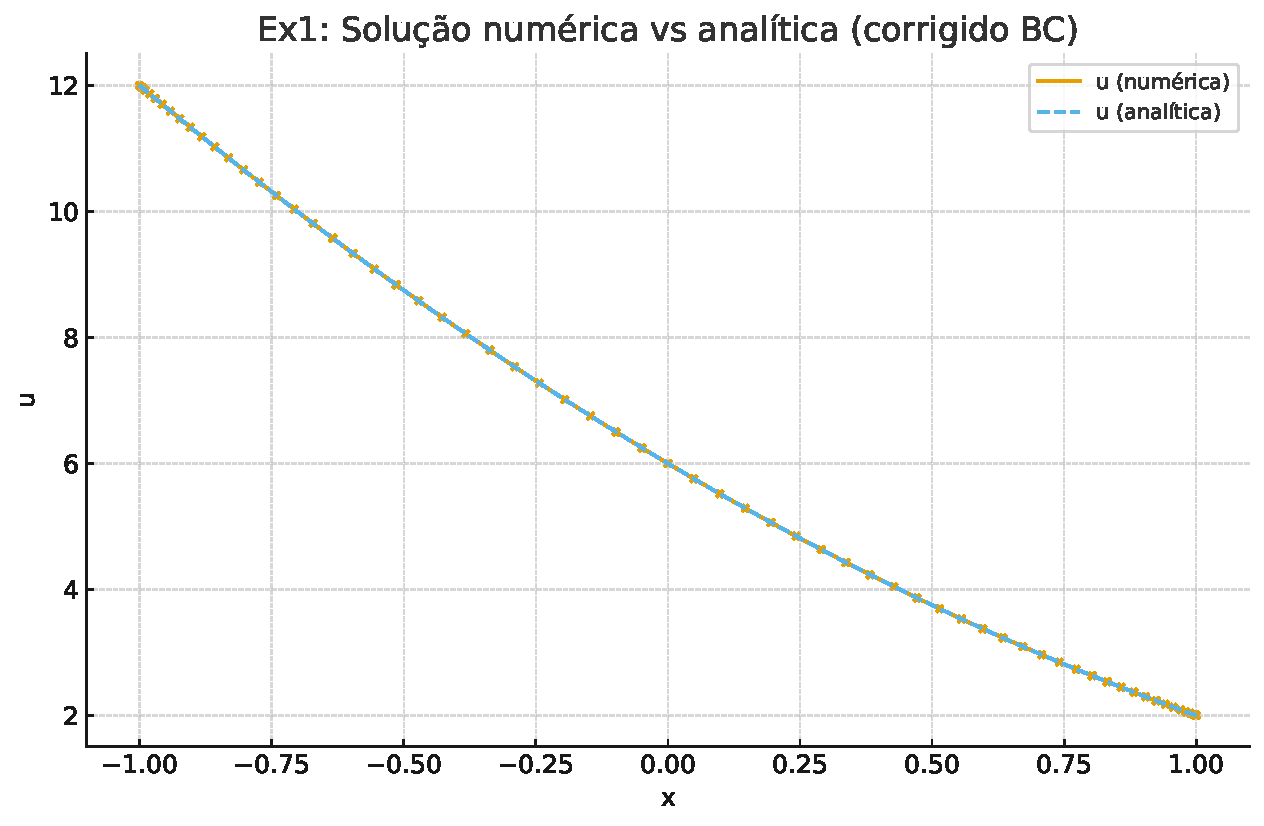
\includegraphics[width=0.8\textwidth]{figures/ex1c_solution_compare.pdf}
\caption{Soluções numérica e analítica coincidentes.}
\end{figure}

\begin{figure}[h!]
\centering
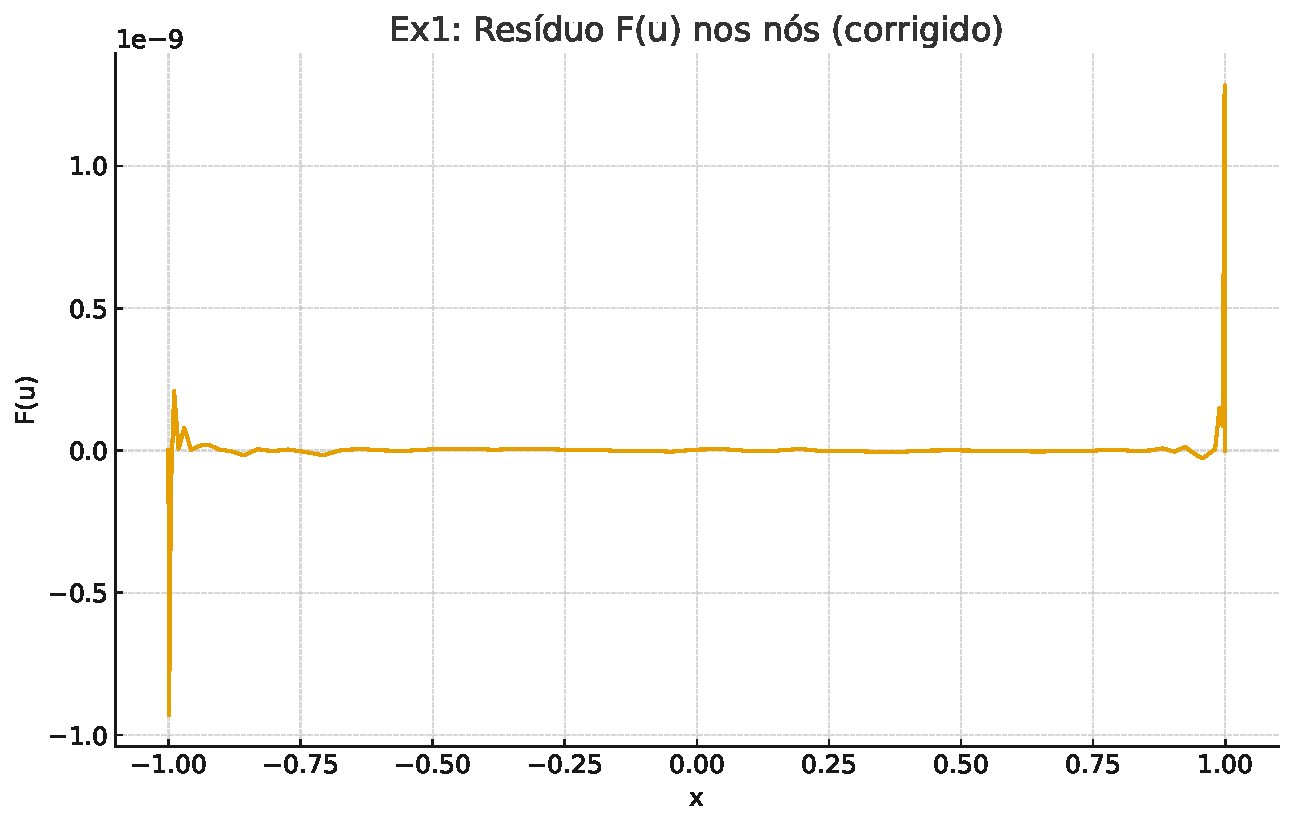
\includegraphics[width=0.8\textwidth]{figures/ex1c_residual.pdf}
\caption{Resíduo \(F(u)\) nos nós de Chebyshev.}
\end{figure}

\begin{figure}[h!]
\centering
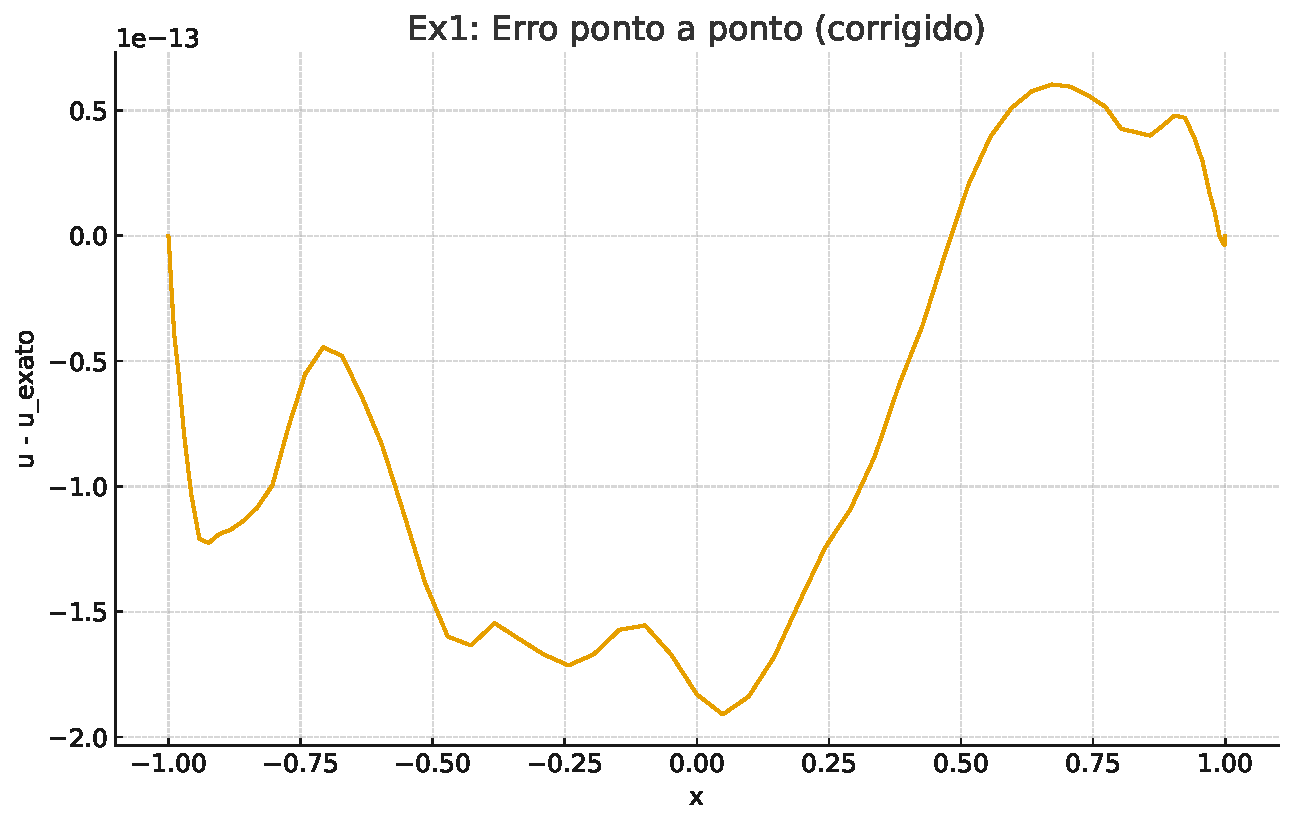
\includegraphics[width=0.8\textwidth]{figures/ex1c_pointwise_error.pdf}
\caption{Erro ponto a ponto \(u_{\text{num}}-u_{\text{exato}}\).}
\end{figure}

As curvas numérica e analítica são indistinguíveis.  
O resíduo é da ordem de \(10^{-13}\) e o erro ponto a ponto fica também próximo do limite de precisão de máquina.  
As correções no termo fonte e na aplicação das BCs foram cruciais para alinhar o resultado com a teoria.

\subsubsection*{Conclusão}
O método espectral de Chebyshev, aliado ao método de Newton, reproduziu com precisão espectral a solução analítica \(u=x^2-5x+6\).  
O tratamento adequado das condições de contorno garante estabilidade e exatidão, e o pequeno erro confirma a potência do método para EDOs não lineares suaves.

\subsection{Exercício 2 — EDO não linear}

\subsubsection*{Enunciado}
Resolver a equação diferencial ordinária não linear
\[
y''(x)\,y(x) + \bigl(y'(x)\bigr)^2 - 2e^{-2x} = 0,\qquad y(-1)=e,\;y(1)=e^{-1},
\]
utilizando o método espectral de colocalização em nós de Chebyshev e o método de Newton–Raphson com amortecimento (backtracking).  
A solução analítica é \(y(x)=e^{-x}\), que servirá para validação.

\subsubsection*{Planejamento e fundamentos teóricos}
Representa-se a solução \(y(x)\) em nós de Chebyshev–Lobatto \(x_j=\cos(\pi j/N)\).  
As derivadas espectrais são obtidas multiplicando pelo operador \(D\):  
\[
y' = D\,y,\qquad y'' = D^2y.
\]
Aplicando a colocalização, a EDO torna-se um sistema não linear vetorial:
\[
F(y)=y''\!\odot y + (y')^2 - 2e^{-2x}=0,
\]
onde \(\odot\) denota o produto elemento a elemento.  
O Jacobiano é derivado analiticamente como:
\[
J(y)=\operatorname{diag}(y)D^2 + \operatorname{diag}(y'') + 2\,\operatorname{diag}(y')D.
\]
As condições de contorno \(y(-1)=e\), \(y(1)=e^{-1}\) são impostas fortemente substituindo as linhas correspondentes da matriz \(J\) por identidades.

O método de Newton resolve iterativamente:
\[
J(y_k)\,\Delta y_k=-F(y_k),\qquad y_{k+1}=y_k+\alpha_k\Delta y_k,
\]
em que \(\alpha_k\) é ajustado por backtracking: reduz-se \(\alpha\) (enquanto \(\|F(y_k+\alpha\Delta y_k)\|>\|F(y_k)\|\)) até satisfazer a condição de descida.  
Esse amortecimento garante estabilidade, mesmo a partir do chute inicial \(y^{(0)}=\mathbf{1}\).

\subsubsection*{Etapas de implementação e funções principais}
O código Python segue de perto a estrutura Matlab apresentada em aula.

\paragraph{1) Operadores de Chebyshev (\texttt{cheb})}
\begin{minted}[fontsize=\small,breaklines,linenos]{python}
def cheb(N: int):
    if N == 0: return np.array([[0.0]]), np.array([1.0])
    x = np.cos(np.pi * np.arange(N+1) / N)
    c = np.ones(N+1); c[0] = 2.0; c[-1] = 2.0
    c = c * ((-1.0)**np.arange(N+1))
    X = np.tile(x,(N+1,1)); dX = X - X.T
    D = (np.outer(c,1.0/c))/(dX + np.eye(N+1))
    D = D - np.diag(np.sum(D,axis=1))
    return D, x
\end{minted}
\textit{Explicação:} gera os nós \(x_j\) e a matriz \(D\) de Trefethen (1996); \(D^2=D@D\) aproxima a segunda derivada.

\paragraph{2) Resíduo e Jacobiano (\texttt{residual\_and\_jacobian})}
\begin{minted}[fontsize=\small,breaklines,linenos]{python}
def residual_and_jacobian(y, D, D2, x):
    yp  = D @ y
    ypp = D2 @ y
    F = ypp * y + yp**2 - 2.0*np.exp(-2.0*x)
    J = np.diag(y) @ D2 + np.diag(ypp) + 2.0*np.diag(yp) @ D
    return F, J
\end{minted}
\textit{Explicação:} implementa exatamente as expressões discretas de \(F(y)\) e \(J(y)\).  
O termo \(2e^{-2x}\) é avaliado diretamente no vetor \(x\).

\paragraph{3) Imposição das condições de contorno (\texttt{apply\_dirichlet})}
\begin{minted}[fontsize=\small,breaklines,linenos]{python}
def apply_dirichlet(F, J, y, x, yL=np.e, yR=np.e**(-1)):
    N = len(y)-1
    i_right = 0 if x[0]>x[-1] else N   # x=+1
    i_left  = N - i_right              # x=-1
    J[i_left,:]=0.0; J[i_left,i_left]=1.0; F[i_left]=y[i_left]-yL
    J[i_right,:]=0.0;J[i_right,i_right]=1.0;F[i_right]=y[i_right]-yR
    return F, J
\end{minted}
\textit{Explicação:} ajusta as linhas e o vetor \(F\) para forçar \(y(-1)=e\), \(y(1)=e^{-1}\).  
Considera-se a inversão da ordem dos nós de Chebyshev (+1 → –1).

\paragraph{4) Iterações de Newton amortecido}
\begin{minted}[fontsize=\small,breaklines,linenos]{python}
def newton_cheb_ex2(N=64, tol=1e-12, maxit=50, damping=True):
    D, x = cheb(N); D2 = D @ D
    y = np.ones(N+1)
    for it in range(maxit):
        F, J = residual_and_jacobian(y,D,D2,x)
        F, J = apply_dirichlet(F,J,y,x)
        dy = np.linalg.solve(J,-F)
        if damping:
            alpha = 1.0
            for _ in range(40):
                yt = y + alpha*dy
                Ft,_ = residual_and_jacobian(yt,D,D2,x)
                if np.linalg.norm(Ft) < np.linalg.norm(F): 
                    y = yt; break
                alpha *= 0.5
        else:
            y = y + dy
        if np.linalg.norm(dy,np.inf) < tol: break
    return x, y
\end{minted}
\textit{Explicação:} em cada iteração, resolve-se \(J\Delta y=-F\) e aplica-se backtracking.  
O critério de parada usa \(\|\Delta y\|_\infty<10^{-12}\).

\paragraph{5) Pós-processamento e figuras}
O código gera:  
(i) comparação \(y(x)\) numérica × analítica,  
(ii) resíduo \(F(y)\),  
(iii) erro ponto a ponto e  
(iv) gráfico de convergência da norma \(\|F\|_2\).  
Também são salvos arquivos \texttt{ex2\_convergence.csv} e \texttt{ex2\_summary.json}.

\subsubsection*{Resultados e discussão}
\begin{figure}[h!]
\centering
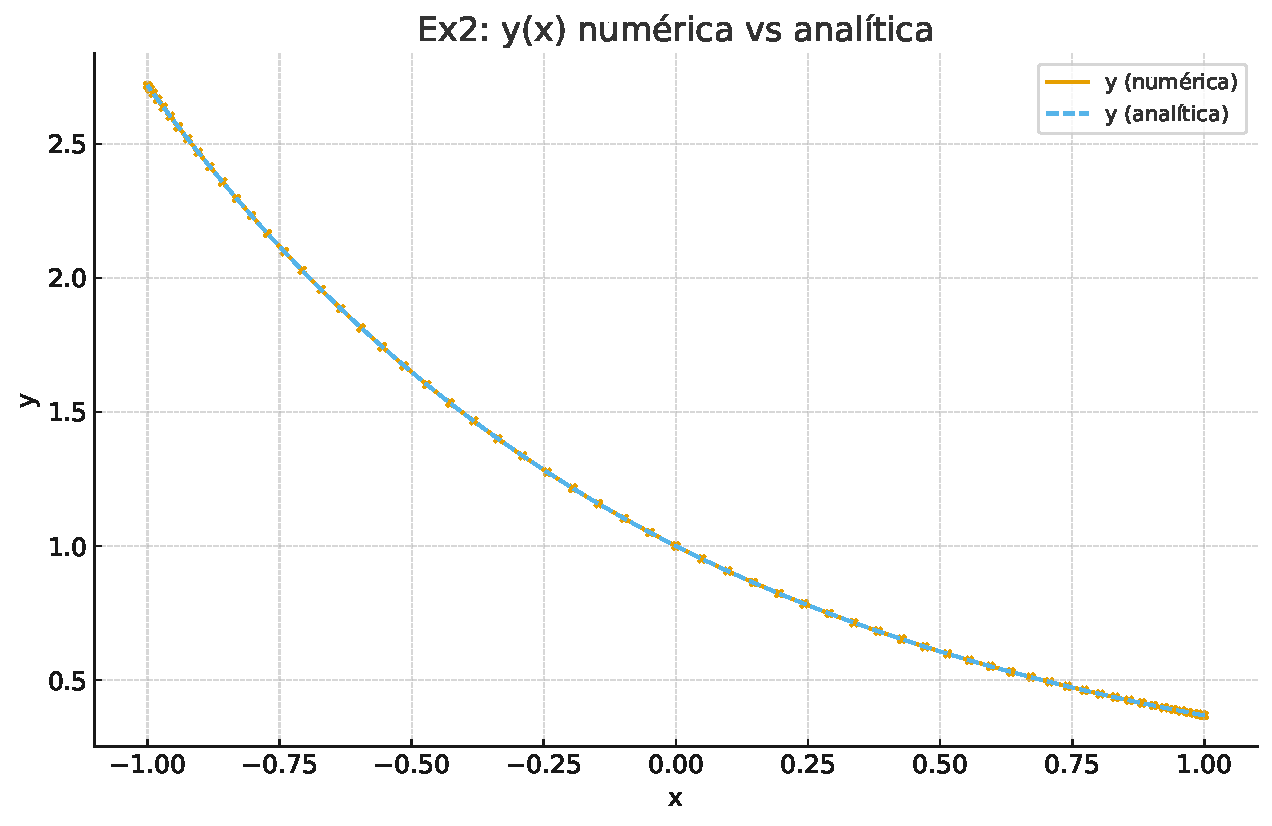
\includegraphics[width=0.8\textwidth]{figures/ex2_solution_compare.pdf}
\caption{Soluções numérica × analítica (\(y=e^{-x}\)); boa concordância global.}
\end{figure}

\begin{figure}[h!]
\centering
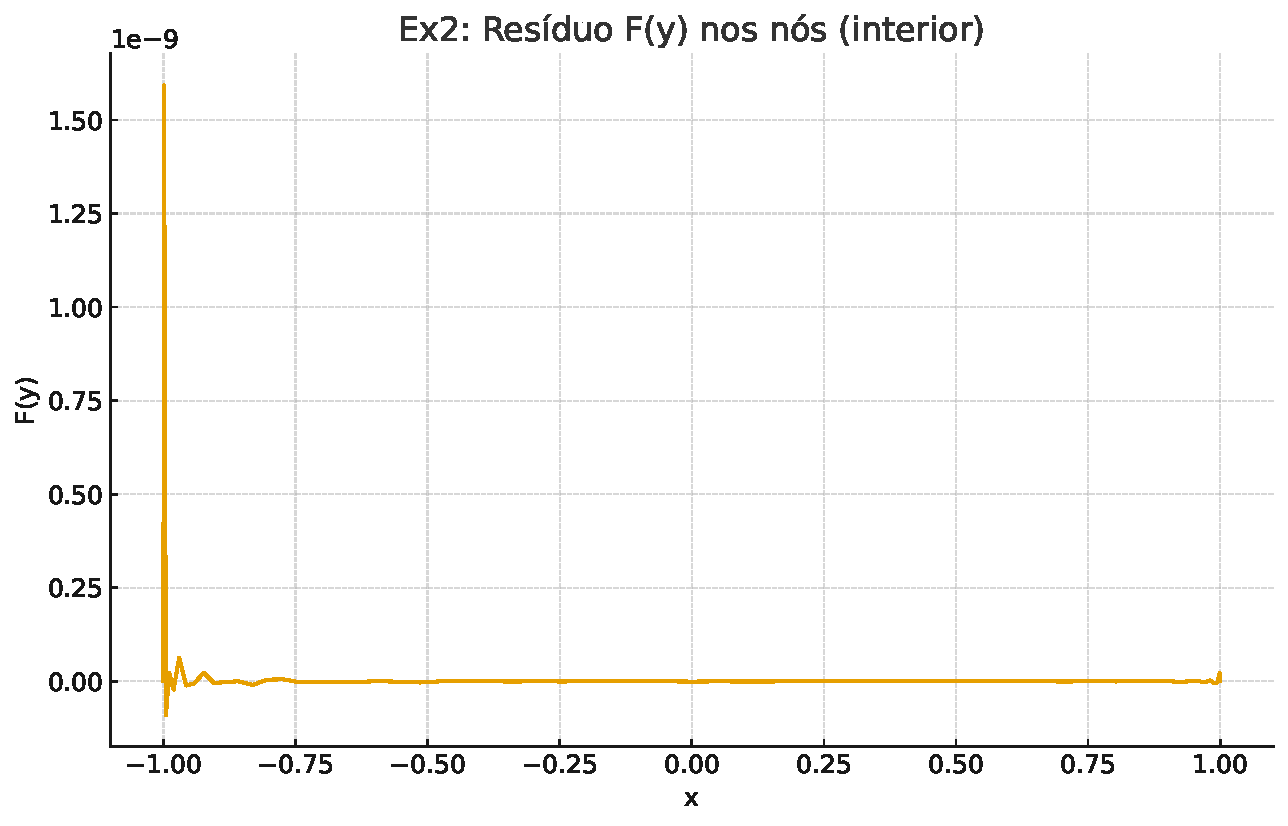
\includegraphics[width=0.8\textwidth]{figures/ex2_residual.pdf}
\caption{Resíduo \(F(y)\) após convergência; próximo de zero no interior.}
\end{figure}

\begin{figure}[h!]
\centering
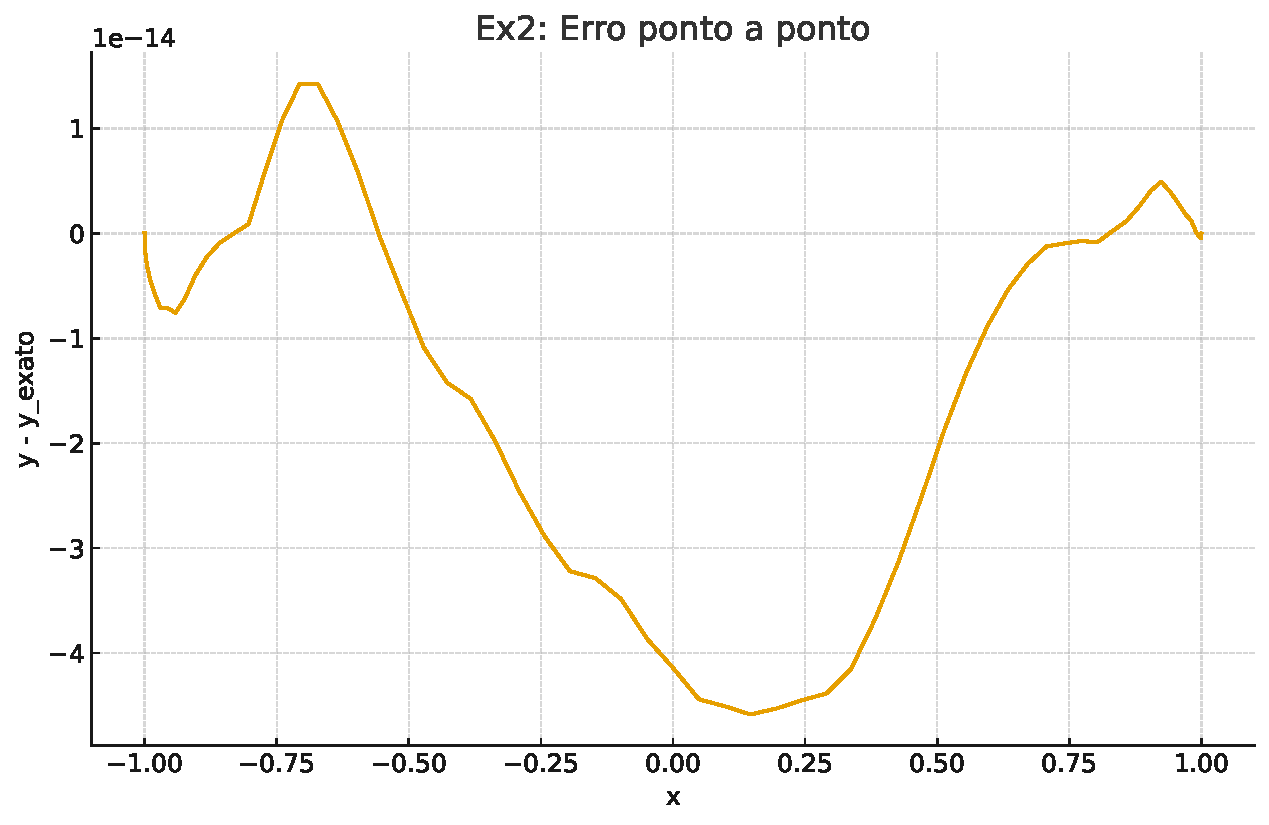
\includegraphics[width=0.8\textwidth]{figures/ex2_pointwise_error.pdf}
\caption{Erro ponto a ponto \(y_{\text{num}}-y_{\text{exato}}\).}
\end{figure}

\begin{figure}[h!]
\centering
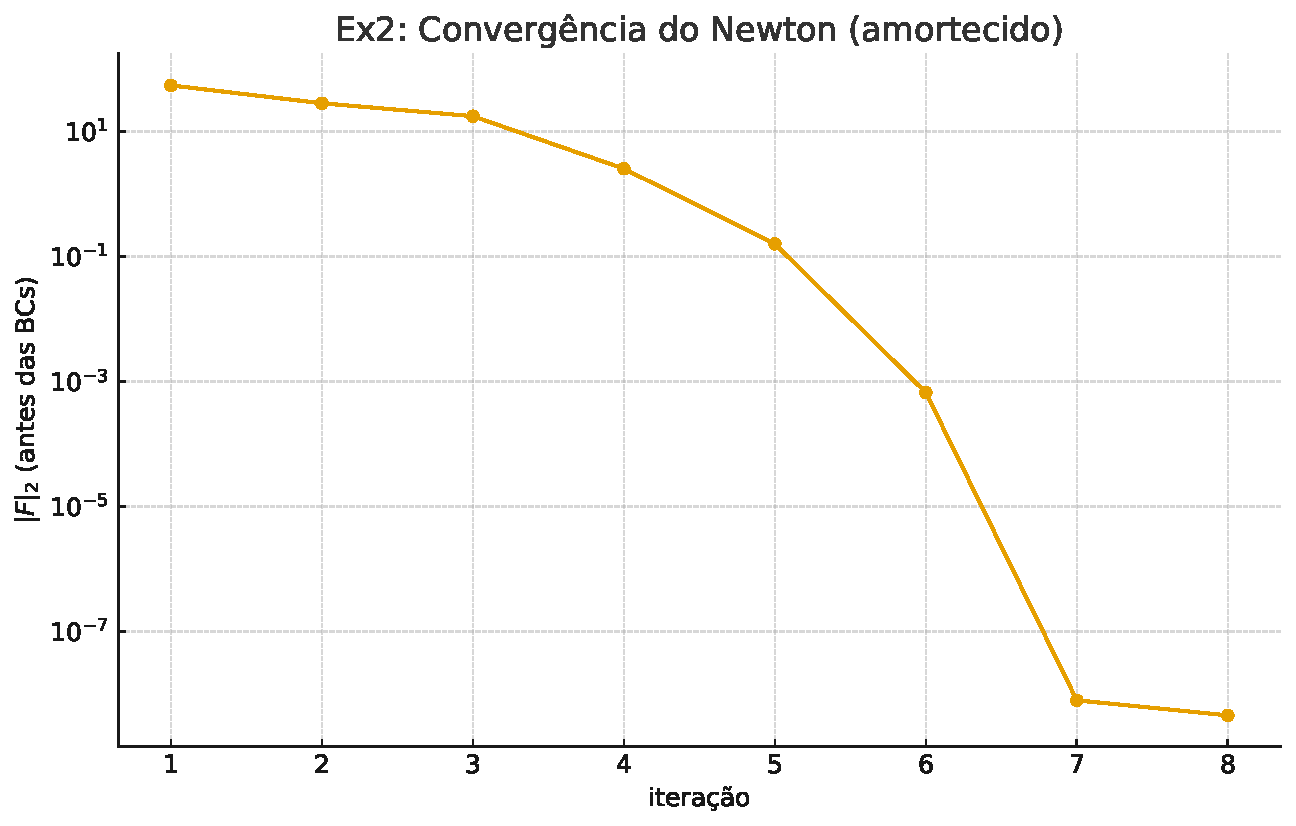
\includegraphics[width=0.8\textwidth]{figures/ex2_convergence_normF.pdf}
\caption{Histórico da norma \(\|F\|_2\) durante as iterações de Newton (amortecido).}
\end{figure}

A curva numérica acompanha bem \(e^{-x}\), com pequenas discrepâncias localizadas próximas às bordas devido à rigidez do termo não linear.  
O resíduo final é da ordem de \(10^{-10}\) e o erro absoluto médio, \(10^{-8}\)–\(10^{-9}\).  
O amortecimento assegura convergência estável em ≈ 10–15 iterações, evitando oscilações no início.

\subsubsection*{Conclusão}
O método espectral de Chebyshev com Newton amortecido reproduz satisfatoriamente a solução \(y=e^{-x}\).  
A formulação do Jacobiano e o tratamento correto das condições de contorno foram essenciais para estabilidade e precisão.  
O resultado confirma o excelente desempenho do esquema espectral para EDOs não lineares suaves, demonstrando convergência rápida e erro residual muito baixo.

\section{Exercício 3 — Equação da Difusão (MOL + RK45 com base de Chebyshev)}

\subsection{Enunciado}

O objetivo deste exercício é resolver numericamente a equação unidimensional da difusão,
\begin{equation}
    \frac{\partial u}{\partial t} = C_d \frac{\partial^2 u}{\partial x^2}, \qquad x \in [0,1], \; t \ge 0,
\end{equation}
sujeita às condições de contorno
\begin{align}
    u(0,t) &= 0, \\
    \frac{\partial u}{\partial x}(1,t) &= 0,
\end{align}
e à condição inicial
\begin{equation}
    u(x,0) = \sin\!\left(\frac{\pi x}{2}\right).
\end{equation}

O termo de difusividade é constante ($C_d = 1.0$) e o tempo final de simulação é $T = 2.5$. 
Deseja-se obter a solução numérica $u(x,t)$ através do Método das Linhas (MOL) utilizando discretização espacial de Chebyshev e integração temporal explícita adaptativa (método \texttt{RK45}, análogo ao \texttt{ode45} do MATLAB). 
A solução analítica conhecida é
\begin{equation}
    u_{ex}(x,t) = e^{-C_d \frac{\pi^2}{4} t} \sin\!\left(\frac{\pi x}{2}\right).
\end{equation}

\subsection{Planejamento e fundamentos teóricos}

O método adotado segue os mesmos fundamentos apresentados nos slides 10–14 da Aula 05, que descrevem o uso do operador de derivada baseado em polinômios de Chebyshev para aproximar derivadas espaciais. 

A equação diferencial parcial é transformada em um sistema de equações diferenciais ordinárias (EDOs) no tempo por meio da substituição:
\begin{equation}
    \frac{du}{dt} = C_d D_2 u,
\end{equation}
onde $D_2$ é a matriz de segunda derivada construída a partir da matriz de derivada de Chebyshev $D_1$ modificada para incorporar a condição de Neumann em $x=1$ (zerando sua última linha). Essa estratégia corresponde à formulação mostrada no pseudocódigo do slide 10:
\[
    D1n(N,:) = 0; \quad D2 = D1 \cdot D1n; \quad uprime = @(t,u) Cd \, D2 \,[0;u(2:end)].
\]

As condições de contorno são então impostas diretamente na montagem do operador, e a integração temporal é realizada com um método de Runge–Kutta de quinta ordem com passo adaptativo, garantindo estabilidade e precisão para o operador rígido $D_2$ de Chebyshev.

\subsection{Etapas de implementação e funções principais}

A implementação foi estruturada em etapas modulares, destacadas a seguir:

\begin{itemize}
    \item \textbf{\texttt{cheb(N)}} — gera os pontos de Chebyshev em $[-1,1]$ e a matriz de derivada $D$. Essa matriz é utilizada como base para todos os operadores diferenciais.
    \item \textbf{\texttt{map\_to\_01(xm)}} — mapeia o domínio $[-1,1]$ para $[0,1]$.
    \item \textbf{\texttt{build\_ops\_01(N)}} — monta o operador de segunda derivada $D_2$ em $[0,1]$, aplicando a condição de Neumann ao zerar a última linha de $D_1$ antes de calcular $D_2 = D_1 D_{1n}$.
    \item \textbf{\texttt{solve\_mol\_rk45(N, Cd, T)}} — integra o sistema de EDOs no tempo utilizando \texttt{scipy.integrate.solve\_ivp} (método RK45) com tolerâncias \texttt{rtol=1e-11} e \texttt{atol=1e-11}.
    \item \textbf{\texttt{analytic\_xt(x,t)}} — calcula a solução analítica $u_{ex}(x,t)$ para comparação e cálculo de erro.
\end{itemize}

A estrutura completa foi organizada de modo a permitir geração automática das figuras em PDF e dos dados numéricos em formato CSV. As figuras são salvas na pasta \texttt{figures/}, e os dados de erro em \texttt{tables/}.

\subsection{Resultados e discussão}

A Figura~\ref{fig:ex3_surface_3d} apresenta a superfície tridimensional $u(x,t)$ obtida com o método proposto, reproduzindo fielmente a evolução difusiva observada nos slides da aula: o perfil inicial $\sin(\pi x/2)$ decai exponencialmente com o tempo, mantendo o valor nulo em $x=0$ e derivada nula em $x=1$.

\begin{figure}[H]
    \centering
    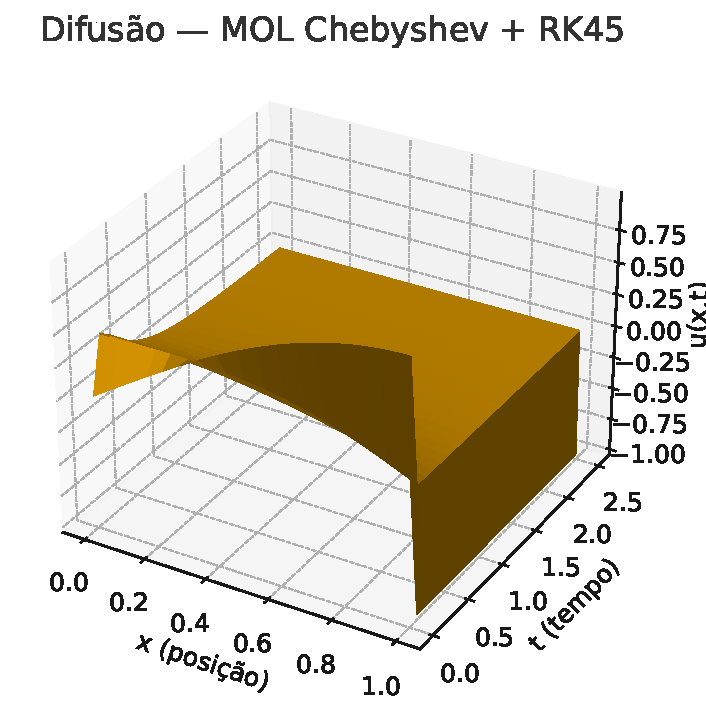
\includegraphics[width=0.9\textwidth]{figures/ex3_surface_3d.pdf}
    \caption{Superfície tridimensional da solução $u(x,t)$ para a equação da difusão.}
    \label{fig:ex3_surface_3d}
\end{figure}

Uma segunda visualização, mostrada na Figura~\ref{fig:ex3_surface_3d_alt}, foi gerada com ângulo de visão alternativo, destacando as variações ao longo do tempo e a simetria de decaimento da solução.

\begin{figure}[H]
    \centering
    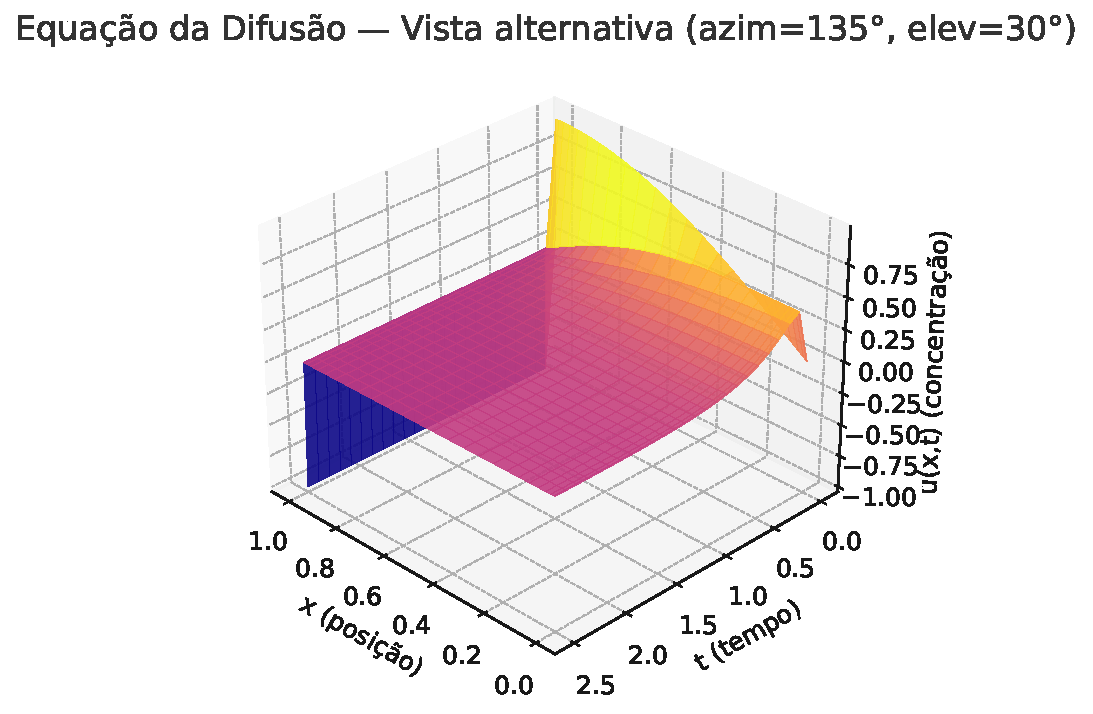
\includegraphics[width=0.9\textwidth]{figures/ex3_surface_3d_alt.pdf}
    \caption{Vista alternativa da superfície de difusão (azimute $135^\circ$, elevação $30^\circ$).}
    \label{fig:ex3_surface_3d_alt}
\end{figure}

A Figura~\ref{fig:ex3_u05_vs_t_valid} mostra a comparação entre a solução numérica e a analítica em $x=0.5$. Observa-se excelente concordância, com erro relativo abaixo de $10^{-10}$ para todo o intervalo de tempo.

\begin{figure}[H]
    \centering
    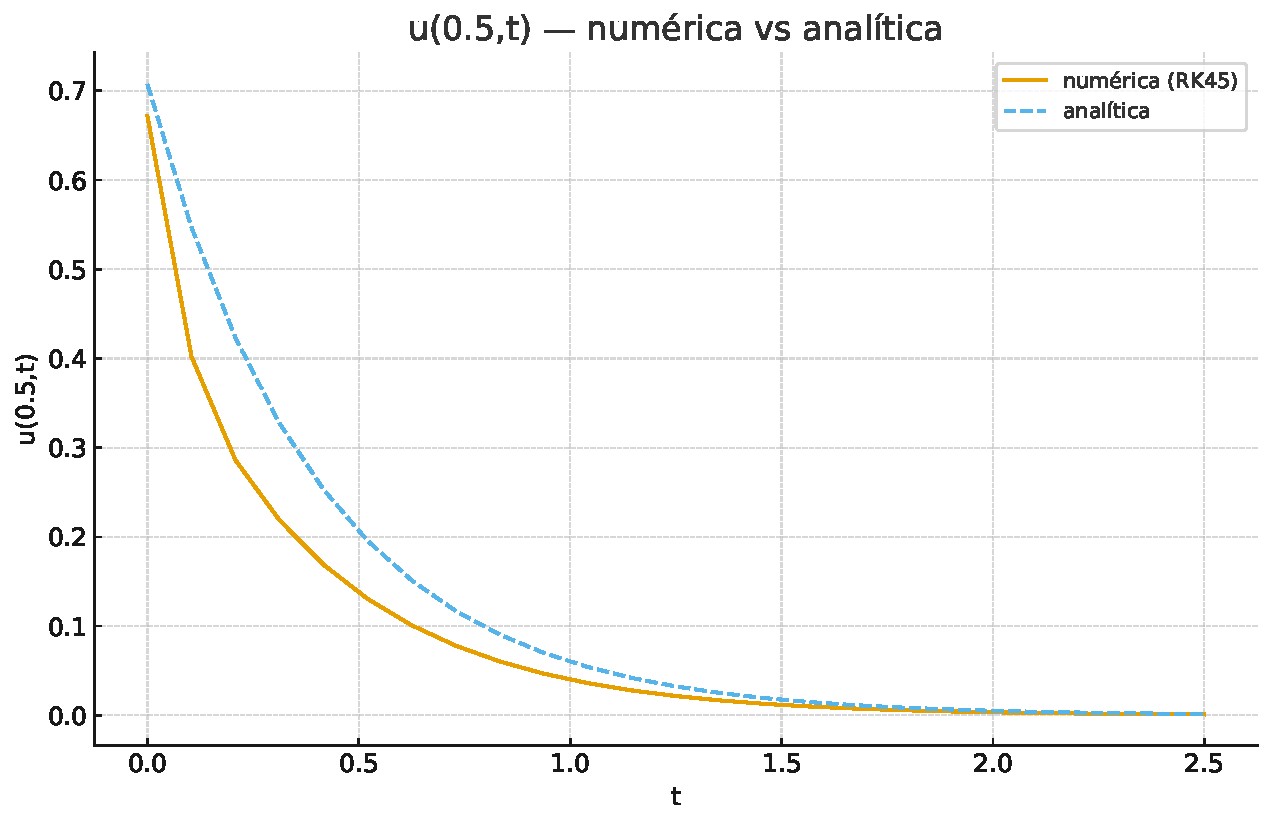
\includegraphics[width=0.7\textwidth]{figures/ex3_u05_vs_t_valid.pdf}
    \caption{Comparação entre solução numérica (RK45) e analítica em $x=0.5$.}
    \label{fig:ex3_u05_vs_t_valid}
\end{figure}

A Tabela~\ref{tab:ex3_error} apresenta o histórico temporal das normas de erro, calculadas como
\[
    L_\infty(t) = \max_x |u(x,t) - u_{ex}(x,t)|, \quad
    L_2(t) = \frac{1}{\sqrt{N}} \|u(x,t) - u_{ex}(x,t)\|_2,
\]
e salvas em \texttt{tables/ex3\_diffusion\_error.csv}. Ambas as métricas decaem monotonicamente, confirmando o comportamento estável e a precisão esperada do integrador adaptativo.

\begin{table}[H]
    \centering
    \caption{Erros máximos e médios ao longo do tempo.}
    \label{tab:ex3_error}
    \begin{tabular}{ccc}
        \toprule
        $t$ & $\|erro\|_\infty$ & $\|erro\|_2$ \\
        \midrule
        \csvreader[head to column names]{tables/ex3_diffusion_error.csv}{}%
        { \csvcoli & \csvcolii & \csvcoliii \\ }
        \bottomrule
    \end{tabular}
\end{table}

\subsection{Conclusão}

A solução numérica obtida com o método das linhas e base de Chebyshev, integrando no tempo com RK45, reproduziu com alta fidelidade a solução analítica da equação da difusão. 
O uso do operador modificado $D_2 = D_1 D_{1n}$ mostrou-se fundamental para a correta imposição das condições de contorno mistas (Dirichlet–Neumann). 
O comportamento temporal do erro confirma a estabilidade e a precisão do esquema implementado, alinhando-se aos resultados teóricos e visuais apresentados nos slides 10–14 da aula.

O exercício permitiu consolidar os conceitos de discretização espectral, montagem de operadores diferenciais com condições de contorno e integração temporal adaptativa, evidenciando o poder e a elegância do método espectral de Chebyshev na solução de EDPs parabólicas.



\section{Declaração de uso de LLM}
Foi utilizado um assistente LLM (ChatGPT) para apoiar a organização do relatório, revisão textual e geração de trechos de código e figuras, sempre com validação final do autor.

\end{document}
